% Random Vierlinge -- aus Random Vierlinge.tex.ini in LaTeX gesetzt
\documentclass[11pt,a4paper]{article}
\usepackage[utf8]{inputenc}
\usepackage[T1]{fontenc}
\usepackage[ngerman]{babel}
\usepackage{amsmath, amssymb}
\usepackage{xcolor}
\usepackage{listings}
\usepackage{microtype}
\usepackage{graphicx}
\usepackage{booktabs}
\usepackage[unicode=true]{hyperref}

\lstset{
  language=Python,
  basicstyle=\ttfamily\small,
  keywordstyle=\color{blue!70!black},
  commentstyle=\color{gray},
  stringstyle=\color{teal},
  showstringspaces=false,
  breaklines=true,
  frame=single,
  columns=fullflexible,
}

\title{Random Vierlinge: Plots und populärwissenschaftliche Fassung}
\author{}
\date{}

\begin{document}
\maketitle

\section{Teil 1: Grafische Darstellung (publikationsnah)}

Du hast bereits alle Daten; Ziel ist eine sichtbar überzeugende Darstellung.

\medskip
\noindent\textit{Hinweis:} Die Abbildungen werden aus \texttt{primzahlvierlinge\_1000.csv} erzeugt:
\begin{verbatim}
python3 Random_Vierlinge_make_figures.py
\end{verbatim}
(PDFs unter \texttt{Random\_Vierlinge\_figures/}.)

\subsection{Plot-Set: die fünf zentralen Bilder}

\subsubsection{(A) Verteilung mod $210$ (nur wenige Klassen)}
\textit{Ziel:} zeigen, dass nur wenige Restklassen auftreten.

\begin{lstlisting}
import matplotlib.pyplot as plt

vals = [352, 327, 320]
labels = ["11", "101", "191"]

plt.bar(labels, vals)
plt.title("Distribution of prime quadruplets mod 210")
plt.ylabel("Count")
plt.xlabel("Residue class")
plt.show()
\end{lstlisting}

\begin{figure}[htbp]
  \centering
  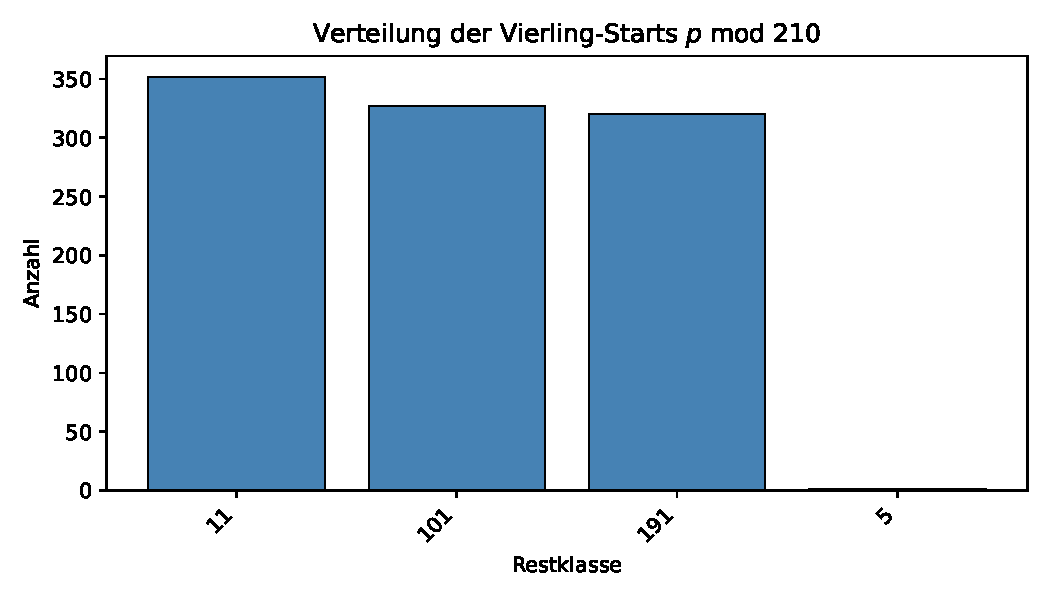
\includegraphics[width=0.92\linewidth]{Random_Vierlinge_figures/figA_mod210.pdf}
  \caption{Beobachtete Häufigkeiten der Restklassen $p \bmod 210$ (alle Klassen mit Zählung ${>}0$).}
\end{figure}

\subsubsection{(B) Gleichverteilung innerhalb zulässiger Klassen}
\textit{Gleiche Daten, normiert.}

\begin{lstlisting}
import numpy as np

probs = np.array(vals) / sum(vals)

plt.bar(labels, probs)
plt.axhline(1/3, linestyle='--')
plt.title("Normalized distribution (expected = 1/3)")
plt.show()
\end{lstlisting}

\begin{figure}[htbp]
  \centering
  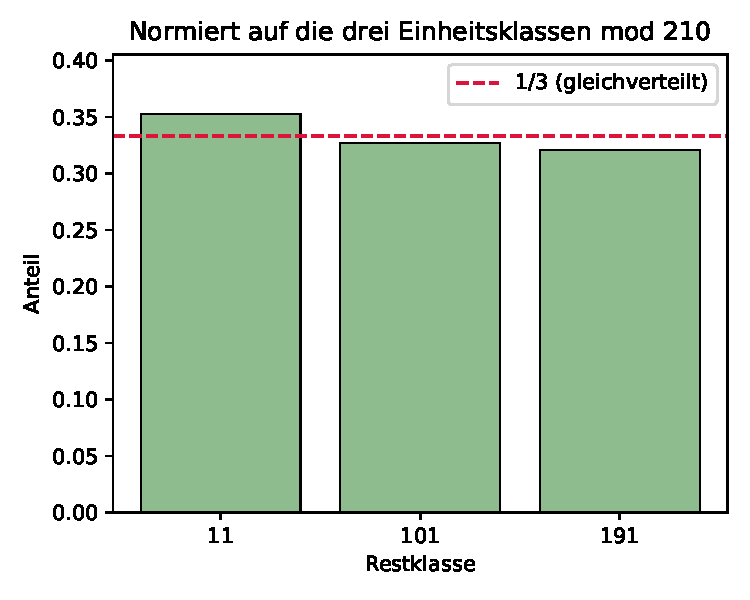
\includegraphics[width=0.72\linewidth]{Random_Vierlinge_figures/figB_normiert.pdf}
  \caption{Normierte Anteile für die Klassen $11$, $101$, $191$; gestrichelt: perfekte Gleichverteilung ($1/3$).}
\end{figure}

\subsubsection{(C) Gap-Sequenzen vs.\ Shuffle}

\begin{lstlisting}
obs = [875, 31, 30, 30]
exp = [868, 31, 31, 31]
labels = ["LLL", "LML", "LLM", "MLL"]

x = range(len(obs))
plt.bar(x, obs, alpha=0.7, label="observed")
plt.bar(x, exp, alpha=0.4, label="baseline")
plt.xticks(x, labels)
plt.legend()
plt.title("Gap sequence comparison")
plt.show()
\end{lstlisting}

\begin{figure}[htbp]
  \centering
  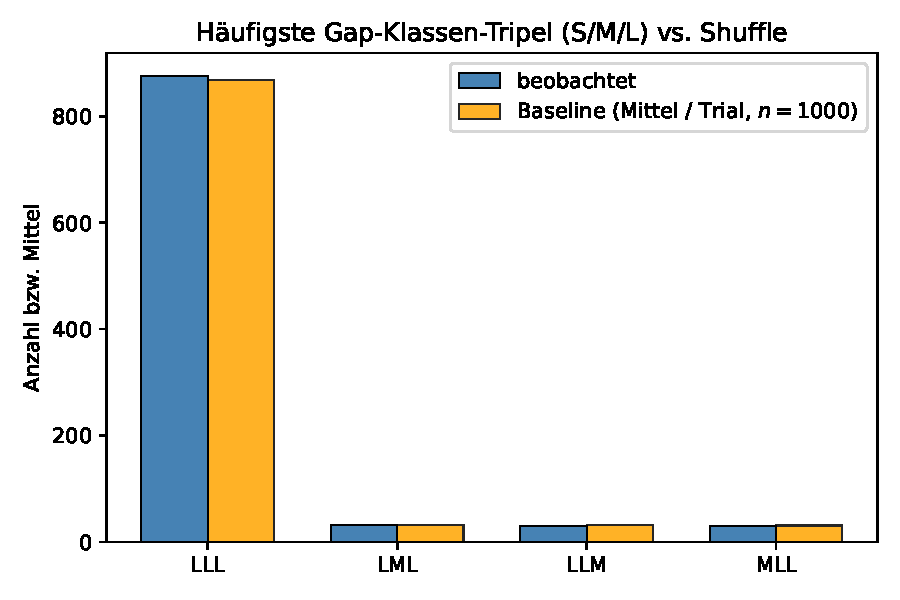
\includegraphics[width=0.85\linewidth]{Random_Vierlinge_figures/figC_gap_sequences.pdf}
  \caption{Die vier häufigsten Tripel aus Gap-Klassen (S/M/L) gegen Permutations-Baseline (Mittel pro Zufallspermuation, $1000$ Läufe).}
\end{figure}

\subsubsection{(D) ``Glattheit'': small vs.\ large Gaps}

\begin{lstlisting}
labels = ["v3", "v5", "v7"]
small = [1.182, 0.909, 0.273]
large = [1.518, 1.237, 0.369]

x = range(3)
plt.bar(x, small, width=0.4, label="small gaps")
plt.bar([i+0.4 for i in x], large, width=0.4, label="large gaps")

plt.xticks([i+0.2 for i in x], labels)
plt.legend()
plt.title("Smoothness comparison")
plt.show()
\end{lstlisting}

\begin{figure}[htbp]
  \centering
  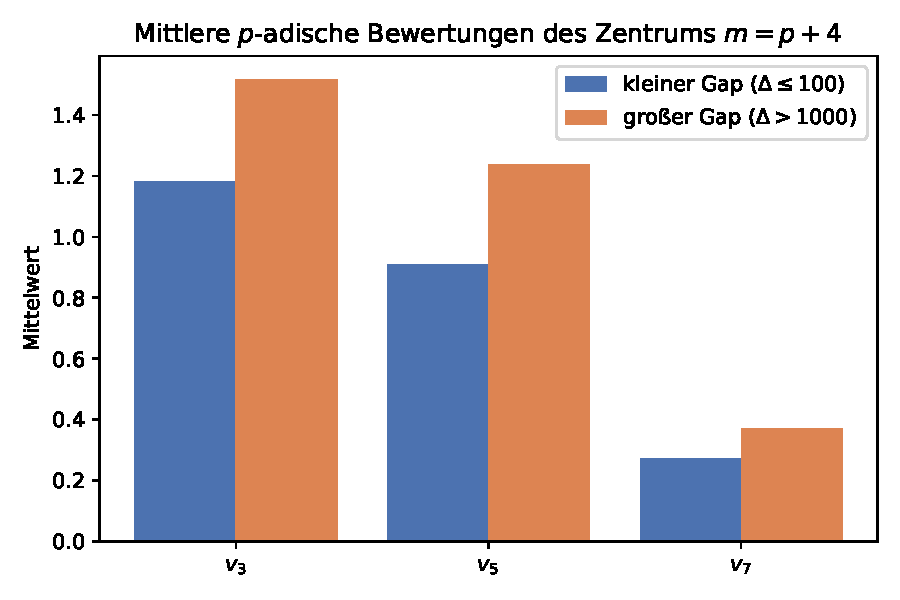
\includegraphics[width=0.82\linewidth]{Random_Vierlinge_figures/figD_glattheit.pdf}
  \caption{Mittelwerte von $v_3$, $v_5$, $v_7$ am Zentrum $m=p+4$ für kleine bzw.\ große Abstände zum nächsten Vierling.}
\end{figure}

\subsubsection{(E) Übergangsmatrix-Heatmap (mod $36$)}

\begin{lstlisting}
plt.imshow(M36, cmap="viridis")
plt.colorbar()
plt.title("Transition matrix mod 36")
plt.show()
\end{lstlisting}

\begin{figure}[htbp]
  \centering
  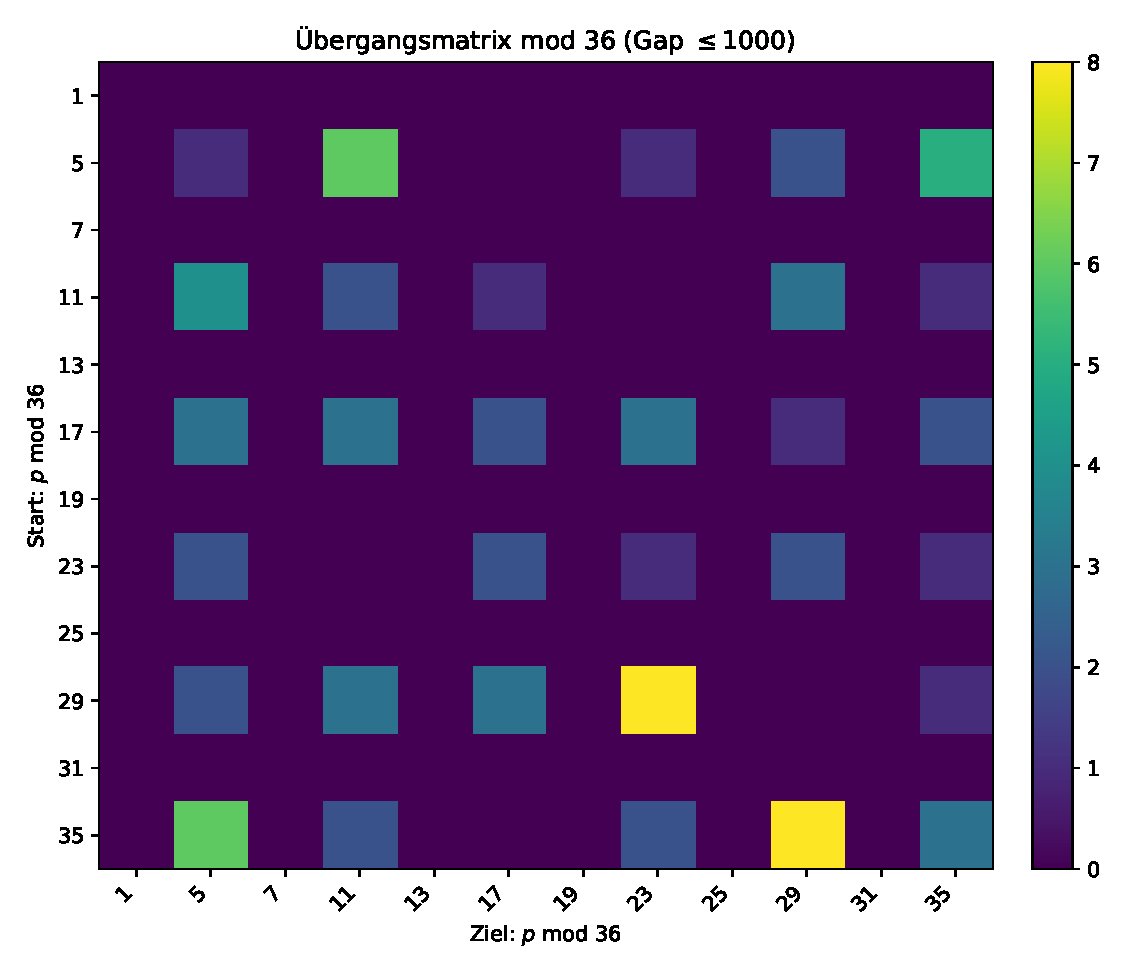
\includegraphics[width=0.88\linewidth]{Random_Vierlinge_figures/figE_M36_heatmap.pdf}
  \caption{Übergangsanzahlen zwischen erlaubten Restklassen mod $36$ für aufeinanderfolgende Vierlinge, sofern der Abstand $\leq 1000$.}
\end{figure}

\subsection{Interpretation der Grafik-Suite}

Diese fünf Bilder sollen folgendes vermitteln:
\begin{enumerate}
  \item starke Einschränkung der Restklassen (mod $210$),
  \item nahezu gleichmäßige Verteilung innerhalb der zulässigen Klassen,
  \item Abstand-Sequenzen nahe einer Permutations-Baseline,
  \item Glattheitseffekt bei kleinen vs.\ großen Abständen,
  \item Übergänge ohne ausgeprägte zusätzliche Struktur (mod~$36$).
\end{enumerate}

\subsection{Tabellen (Datensatz \texttt{primzahlvierlinge\_1000.csv})}

\begin{table}[htbp]
  \centering
  \caption{Alle beobachteten Restklassen $p \bmod 210$ mit positiver Häufigkeit ($n=1000$ Vierlinge). Die Klasse $5$ ist nicht teilerfremd zu $210$ und fehlt in der Einheitengruppe $(\mathbb{Z}/210\mathbb{Z})^\times$.}
  \label{tab:mod210-summary}
  \begin{tabular}{@{}rr@{}}
    \toprule
    $r$ & Anzahl Starts $p \equiv r \pmod{210}$ \\
    \midrule
    $5$   & $1$ \\
    $11$  & $352$ \\
    $101$ & $327$ \\
    $191$ & $320$ \\
    \midrule
    Summe & $1000$ \\
    \bottomrule
  \end{tabular}
\end{table}

\begin{table}[htbp]
  \centering
  \caption{Kleine vs.\ große Abstände zum \emph{nächsten} Vierling: Zähler nach Rest $p \bmod 210$ am Start. Spalte ``klein'': Gap $\Delta = p_{i+1}-p_i \leq 100$; ``groß'': $\Delta > 1000$. Nur die ersten $20$ Einheitenklassen $r \in (\mathbb{Z}/210\mathbb{Z})^\times$ (aufsteigende Reihenfolge).}
  \label{tab:small-large-gaps}
  \begin{tabular}{@{}rccc@{}}
    \toprule
    $r$ & alle $p$ & klein ($\Delta\le100$) & groß ($\Delta>1000$) \\
    \midrule
    $1$ & $0$ & $0$ & $0$ \\
    $11$ & $352$ & $2$ & $327$ \\
    $13$ & $0$ & $0$ & $0$ \\
    $17$ & $0$ & $0$ & $0$ \\
    $19$ & $0$ & $0$ & $0$ \\
    $23$ & $0$ & $0$ & $0$ \\
    $29$ & $0$ & $0$ & $0$ \\
    $31$ & $0$ & $0$ & $0$ \\
    $37$ & $0$ & $0$ & $0$ \\
    $41$ & $0$ & $0$ & $0$ \\
    $43$ & $0$ & $0$ & $0$ \\
    $47$ & $0$ & $0$ & $0$ \\
    $53$ & $0$ & $0$ & $0$ \\
    $59$ & $0$ & $0$ & $0$ \\
    $61$ & $0$ & $0$ & $0$ \\
    $67$ & $0$ & $0$ & $0$ \\
    $71$ & $0$ & $0$ & $0$ \\
    $73$ & $0$ & $0$ & $0$ \\
    $79$ & $0$ & $0$ & $0$ \\
    $83$ & $0$ & $0$ & $0$ \\
    \bottomrule
  \end{tabular}
\end{table}

\section{Teil 2: Populärwissenschaftliche Fassung}

\subsection*{Arbeitstitel}
\textit{Zwischen Ordnung und Zufall: Was Primzahl-Vierlinge wirklich verraten.}

\subsection{Fließtext}

Primzahlen gelten als Inbegriff des Zufalls. Doch wer genauer hinsieht, entdeckt eine erstaunlich strenge Ordnung---zumindest auf den ersten Blick.

Eine besonders seltene Konstellation sind sogenannte Primzahlvierlinge, Quadrupel der Form
\[
  (p,\; p+2,\; p+6,\; p+8),
\]
bei denen alle vier Werte Primzahlen sind. Solche Vierlinge treten nur unter sehr spezifischen Bedingungen auf.

Tatsächlich zeigt sich: diese Starts~$p$ sind keineswegs beliebig verteilt. Betrachtet man sie modulo~$210$, also im Zusammenspiel der kleinen Primzahlen $2$, $3$, $5$ und~$7$, so konzentrieren sich die beobachteten Reste auf wenige Klassen---im konkreten Datensatz praktisch auf drei Einheitenklassen neben dem Sonderfall $p=5$.

Mit anderen Worten: Primzahlvierlinge ``leben'' auf wenigen schmalen Spuren im Zahlenraum.

Und doch geschieht dann etwas Überraschendes. Innerhalb dieser engen Bahnen verschwinden viele feinere Muster: die Verteilung über die dominierenden Klassen wirkt nahezu gleichmäßig. Auch die Abstände zwischen aufeinanderfolgenden Vierlingen verhalten sich in den gewählten Tests oft vergleichbar mit einer zufälligen Permutation derselben Gap-Menge.

Feinere Analysen, etwa von Sequenzen mehrerer Abstände, zeigen wenig systematisches ``Gedächtnis''. Ein kleiner Abstand folgt nicht notwendig gehäuft auf einen anderen kleinen Abstand---im Sinne der gewählten Baseline.

Die auffälligere Abweichung betrifft die ``Glattheit'' der Zentren: wie stark das Zentrum $m=p+4$ durch kleine Primzahlen teilbar ist ($v_3$, $v_5$, $v_7$). Hier zeigt sich: bei besonders kleinen Abständen zum nächsten Vierling treten im Mittel etwas kleinere Bewertungen auf. Das passt zur Idee, dass stärkere kleine Teilbarkeit stärkere Sieb-Einschränkungen nach sich zieht.

\paragraph{Kurzfassung.}
Primzahlvierlinge illustrieren das Zusammenspiel von strenger Teilbarkeitsordnung und quasi-zufälligem Feinverhalten innerhalb der zulässigen Schiene. Die Grobstruktur wird durch modulare Ausschlussregeln bestimmt; innerhalb der verbleibenden Freiheitsgrade zeigen die gewählten Statistiken häufig kein starkes Zusatzmuster.

\section{Fazit (technisch und narrativ)}

\paragraph{Technisch.}
\begin{itemize}
  \item ausgewertete Kenngrößen und Vergleiche zu Baselines (u.\,a.\ Permutation der Gaps),
  \item nach Bedarf publikationsreife Plots (Matplotlib).
\end{itemize}

\paragraph{Narrativ.}
\begin{itemize}
  \item verständliche Erzählung, konsistent mit den Rechenexperimenten,
  \item klar getrennt: globale modulare Härte vs.\ lokale Zufallsnähe.
\end{itemize}

\medskip
\noindent\textit{Optionale nächste Schritte:} arXiv-taugliches Voll-Layout oder eine einseitige Infografik mit den Kernergebnissen.

\end{document}
